\documentclass[mathserif]{beamer}
\usepackage{movie15}
\usepackage{psfrag,graphicx}
\usepackage{amsmath}
\graphicspath{{figs/}}

\usetheme{Boadilla}
\makeatother
\setbeamertemplate{footline}[frame number]

\usepackage{graphicx}
\usepackage{caption}
\usepackage{subcaption}
\captionsetup{compatibility=false}
\usepackage{amsmath} 
\usepackage{amssymb} 
\usepackage{amsthm}  
\usepackage{bm}
\usepackage{lipsum}
\usepackage[linesnumbered, ruled]{algorithm2e}
\usepackage{color}
\newtheorem{assumption}{Assumptions}
\newtheorem{prop}{Proposition}
\newtheorem{defn}{Definition}
\newtheorem{thm}{Theorem}
\newtheorem{lem}{Lemma}
\newtheorem{cor}{Corollary}
\newtheorem{sol}{Decentralized Solution}
\newtheorem{thresh}{$\epsilon$-thresholding}
\definecolor{light-gray}{gray}{0.8}
\usepackage{textcomp}

\newcommand{\backupbegin}{
   \newcounter{finalframe}
   \setcounter{finalframe}{\value{framenumber}}
}
\newcommand{\backupend}{
   \setcounter{framenumber}{\value{finalframe}}
}
\newcommand{\norm}[1]{\left\lVert #1 \right\rVert}

\makeatletter
\setbeamertemplate{navigation symbols}{}
\title{Class Ten: Model Selection, Part two}

\author{{ER290: Data, Energy and Justice\\  Instructor: Duncan Callaway} \\
}
\institute{University of California, Berkeley}
\date{Fall 2017}
\begin{document}

\frame{
  \titlepage
}


\begin{frame}{Recap Thursday's lecture objectives}
\begin{itemize}
\item Refine our understanding of model identification as an optimization problem
\uncover<2->{\begin{align*}
\min_\beta \sum_{i=1}^N \left(Y_i - X_i \beta \right)^2+\lambda \cdot R(\beta)\end{align*}}
\item Learn how to adjust errors to compare models with different $p$
\begin{itemize}
\item<3-> k-fold cross validation, AIC, BIC, adjusted R$^2$...
\end{itemize}
\item Understand what ``regularization'' is and why we do it
\begin{itemize}
\item<4-> A tool for adapting optimization problems to be well behaved
\item<4-> In ML, a tool to tradeoff bias and variance 
\item<4-> Something that causes you to solve a different problem than the original $\rightarrow$ parameter bias
\end{itemize}
\item Understand tradeoffs between subset selection, ridge and lasso
\begin{itemize}
\item<5-> Speed (fastest to slowest): Ridge, Lasso, Subset
\item<5-> Subset selection and Lasso do feature selection.  Ridge does not.
\item<5-> You can naturally tune prediction bias-variance with Ridge and Lasso
\end{itemize}
\end{itemize}
\end{frame}

\begin{frame}{A bit more recap}

The regularizing term, $R(\beta)$ can take a lot of forms.//~//

We looked at
\begin{align*}
R(\beta)  &=\sum_{i=1}^K I(\beta_i) &= \norm{\beta}_0\quad &\text{(subset selection)}\\
R(\beta)  &=\sum_{i=1}^K |\beta_i| &= \norm{\beta}_1\quad &\text{(lasso)}\\
R(\beta) &=\sum_{i=1}^K \beta_i^2 &\quad &\text{(ridge)}
\end{align*}

Note, last time I erroneously referred to $\sum_{i=1}^K \beta^2$ as the 2-norm.  It's not!  ($\norm{\beta}_2 = \sqrt{\sum_{k=1}^K \beta^2}$ is.)

\end{frame}


\begin{frame}{Ok, how do you do it?}
We're looking at three kinds of methods in Ch 6 (last lecture and today):
\begin{itemize}
\item Subset selection -- last time
\item Shinkage -- last time
\item Dimension reduction -- today\\~\\
\end{itemize}

{\large \color{blue} Today's Objectives}
\begin{itemize}
\item Revisit intuition for ridge and lasso
\item Look at a few examples for what happens to ``shrunk'' parameter estimates (revisit from last time)
\item Understand the basic concepts of dimension reduction -- why we do it and how it works
\item Set up thursday discussion about the role of prediction in policy problems.
\end{itemize}
\end{frame}

\begin{frame}{Fixing intuition about why lasso selects features, part 1}

First, recognize that the formulations for ridge and lasso I presented are Lagrangian versions of constrained optimization problems:

\begin{align*}
\min_\beta \sum_{i=1}^N \left(Y_i - X_i \beta \right)^2+\lambda \cdot \sum_{k=1}^K \beta_k^2 
\Leftrightarrow
\uncover<2->{\begin{cases}
\min_\beta \sum_{i=1}^N \left(Y_i - X_i \beta \right)^2\\
\text{subject to}\\
\sum_{k=1}^K \beta_k^2 \le s
\end{cases}}
\end{align*}

\begin{align*}
\min_\beta \sum_{i=1}^N \left(Y_i - X_i \beta \right)^2+\lambda \cdot \sum_{k=1}^K |\beta_k|
\Leftrightarrow
\uncover<2->{\begin{cases}
\min_\beta \sum_{i=1}^N \left(Y_i - X_i \beta \right)^2\\
\text{subject to}\\
\sum_{k=1}^K |\beta_k | \le s
\end{cases}}
\end{align*}

\end{frame}

\begin{frame}{Fixing intuition about why lasso selects features, part 2}
\begin{columns}
\column{0.3\textwidth}
Lines centered on $\hat{\beta}$ are RSS ``contours'' \\~\\

Shapes at the origin: boundaries of regions defined by the inequality constraints \\~\\

For a given $s$ (constraint contour), the RSS contour closest to $\hat{\beta}$ wins\\~\\

\column{0.7\textwidth}
\begin{figure}
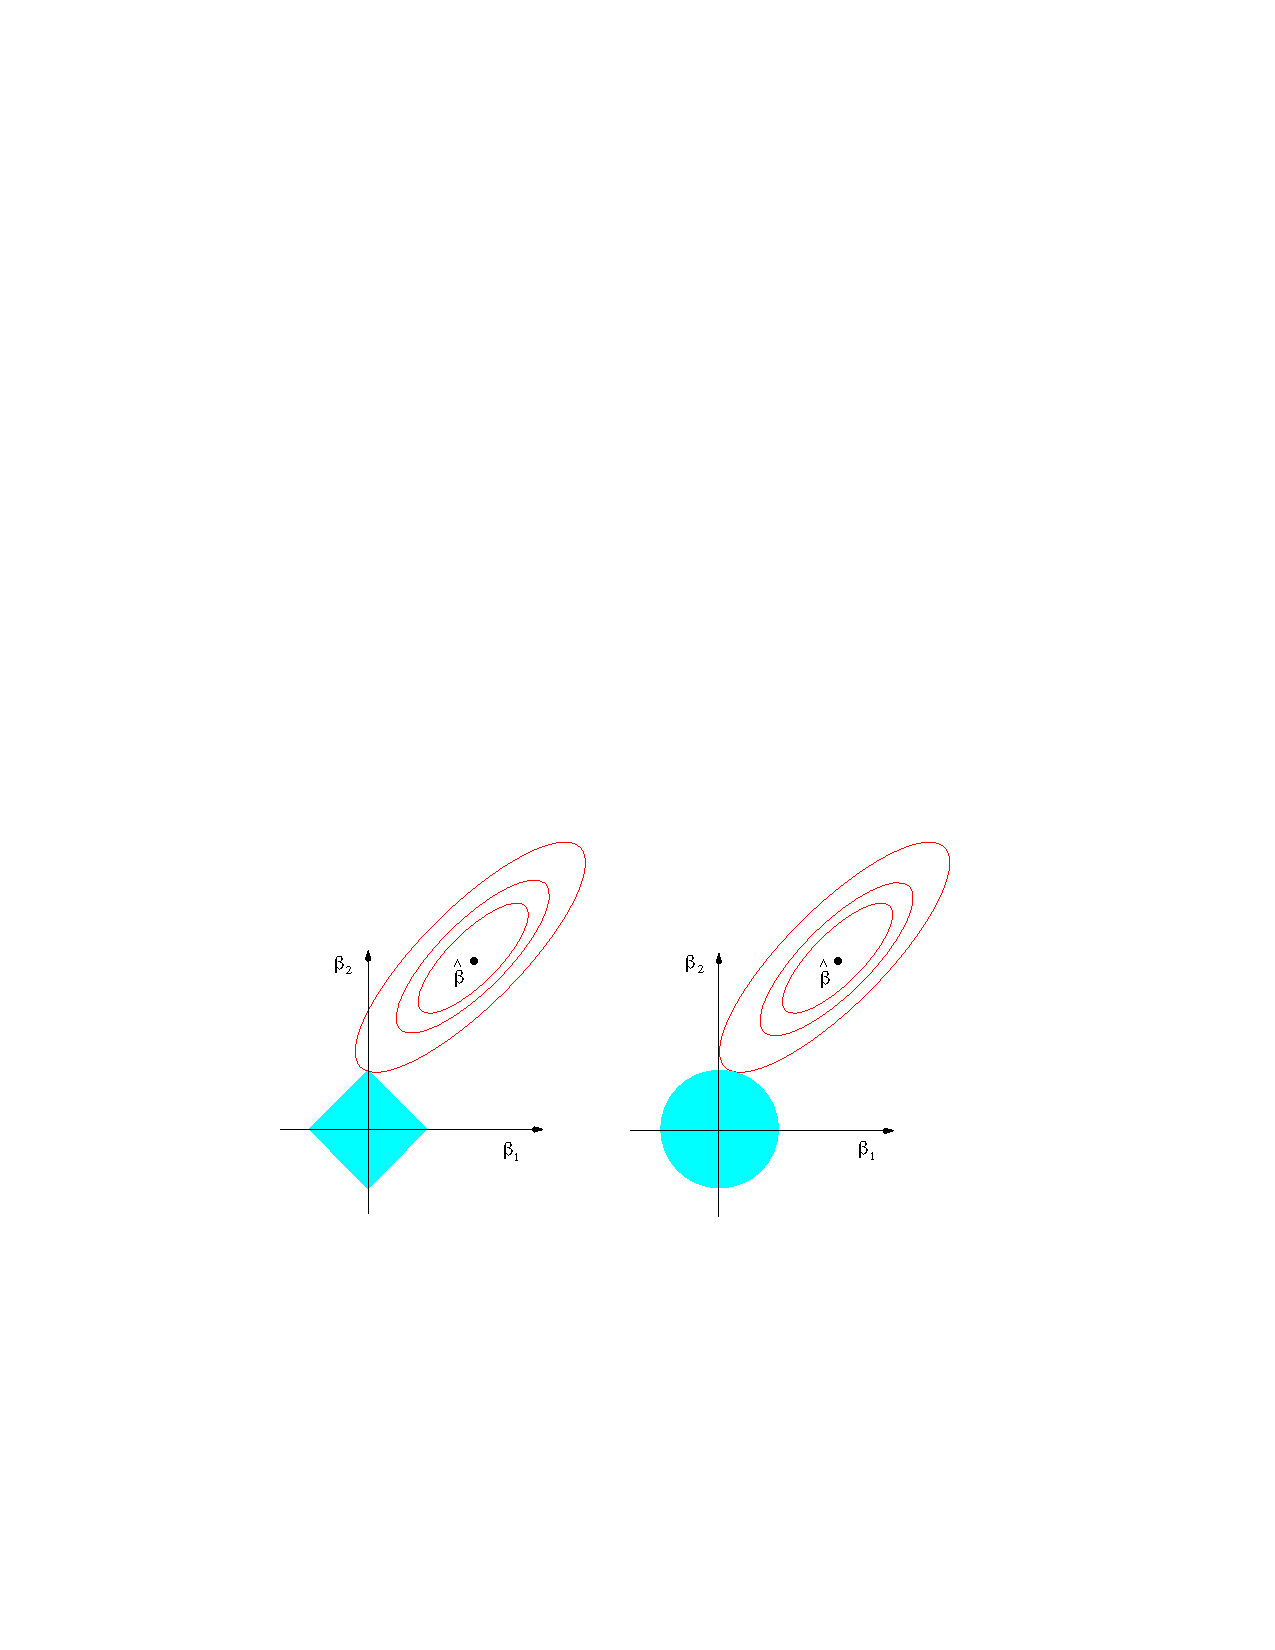
\includegraphics[scale=0.7]{lasso_v_ridge}
\caption*{\tiny Figure taken from Elements of Statistical Learning}
\end{figure}
\end{columns}


For lasso, you can see this is much more likely to happen at a corner (one parameter zero) than it is for ridge

\end{frame}

\begin{frame}{What do the parameter estimates look like?}

\begin{figure}
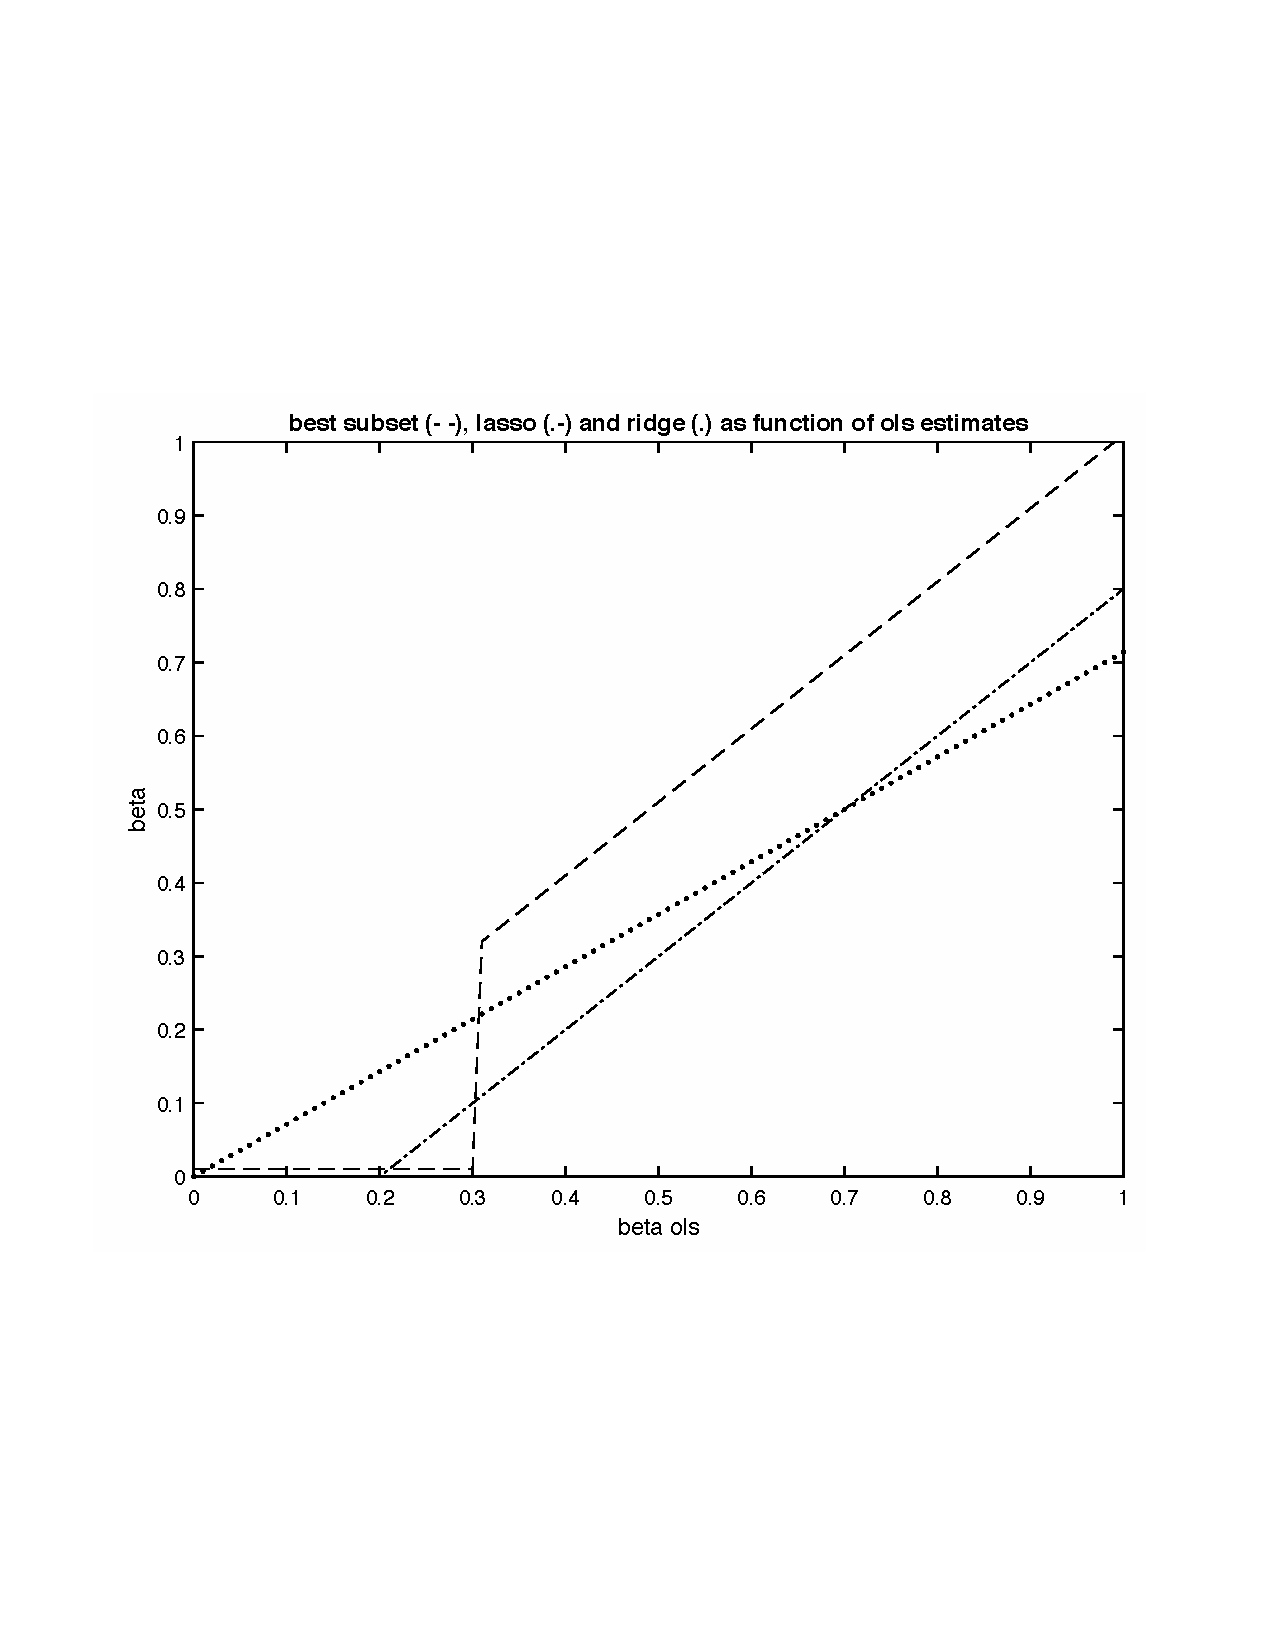
\includegraphics[scale=0.5]{lasso-ridge-subset-vs-ols}
\caption*{\tiny Figure taken from Imbens 2015 NBER lecture}
\end{figure}

\end{frame}

\begin{frame}{Lasso or ridge?}


\begin{columns}
\column{0.5\textwidth}
Simulated data set from $n=50$ and $p=45$.  The response is a function of all 45 predictors.  Figure shows test MSE on y-axis.\\~\\
\begin{figure}
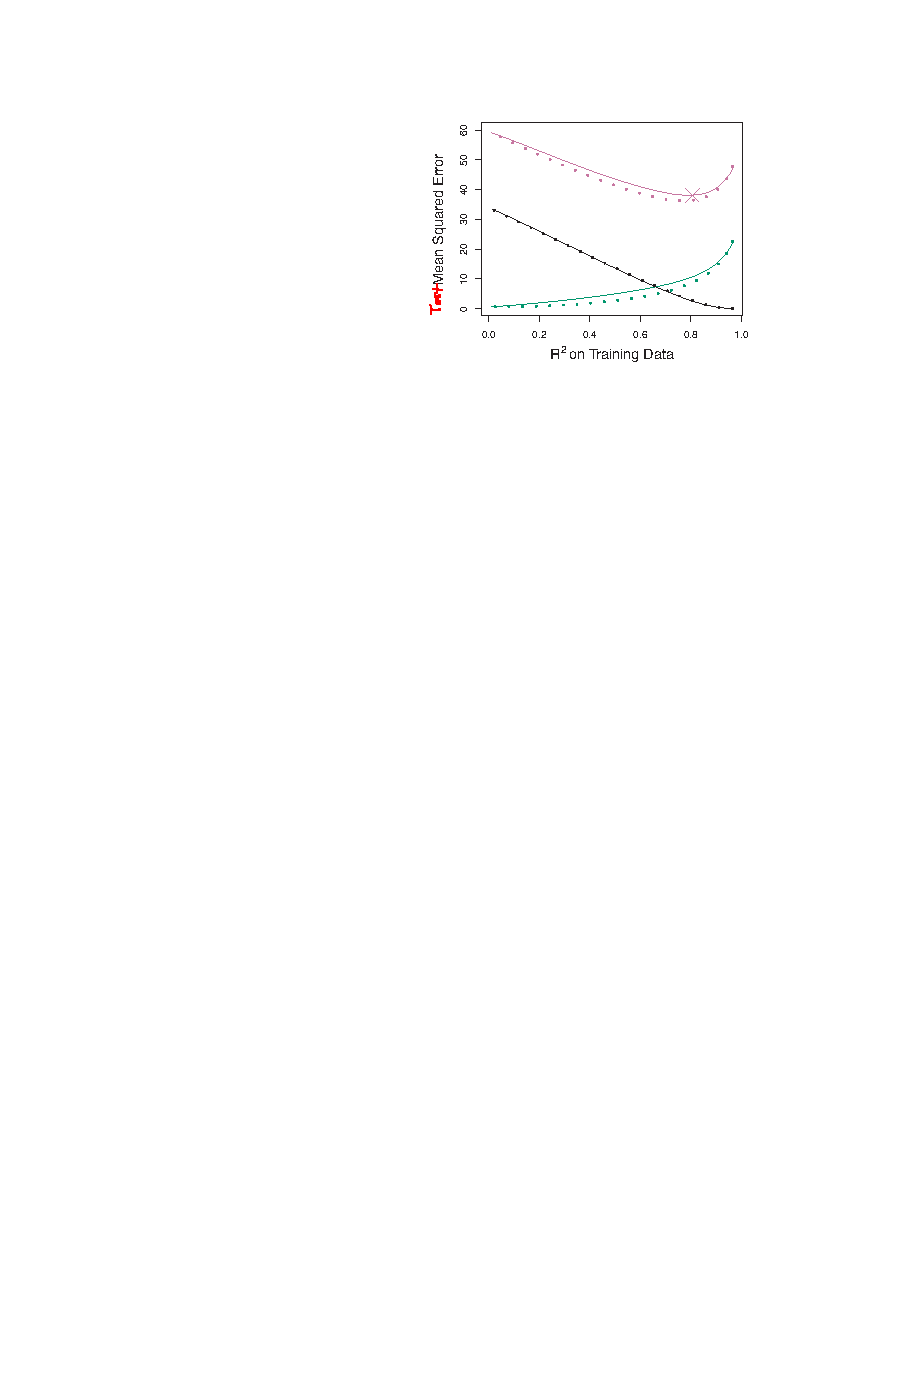
\includegraphics[scale=1]{lasso-v-ridge-45variables}
\end{figure}

\column{0.5\textwidth}
Simulated data set from $n=50$ and $p=45$.  The response is a function of only 2 of the 45 predictors.  Figure shows test MSE on y-axis.\\~\\
\begin{figure}
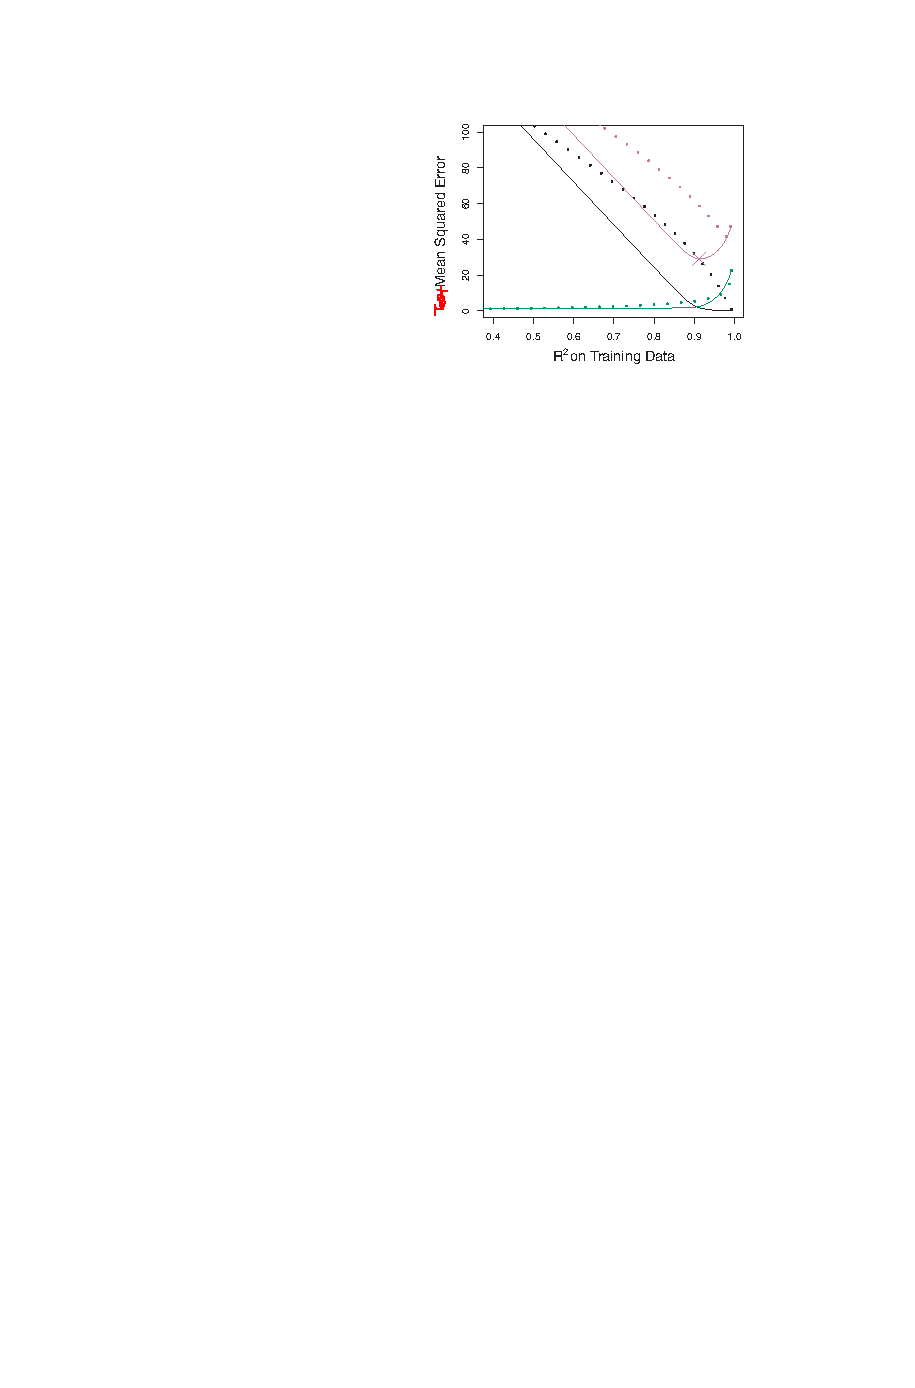
\includegraphics[scale=1]{lasso-v-ridge-2variables}
\end{figure}

\end{columns}

Red show total MSE.  (Black and green are variance and bias.) Dashed line -- best Ridge.  Solid line -- best lasso.  
\end{frame}

\begin{frame}{Lasso or ridge?}

Lasso performs better when the number of predictors truly is small, and otherwise it performs worse.  \\~\\

Since you can't know ahead of time if the response is a function of a few or all predictors, it makes sense to just try both.  

\end{frame}


\begin{frame}{Choosing $\lambda$}

As we've seen, $\lambda$ can take a range of values.  Here we see the tradeoff for the 2-of-45 predictors example  lasso example from two slides ago. 


\begin{figure}
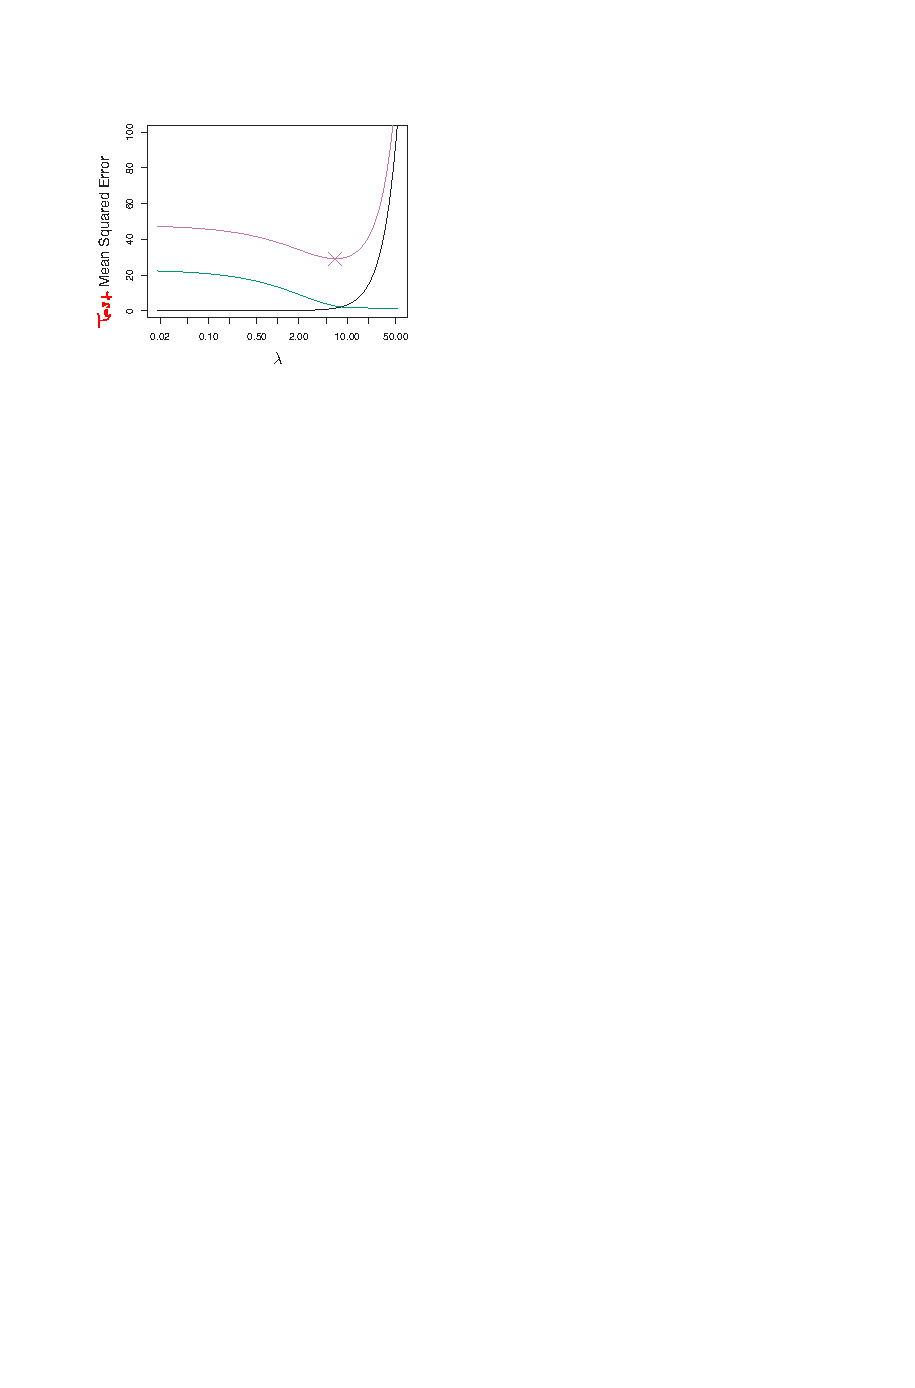
\includegraphics[scale=.7]{bias-variance-lasso-2}
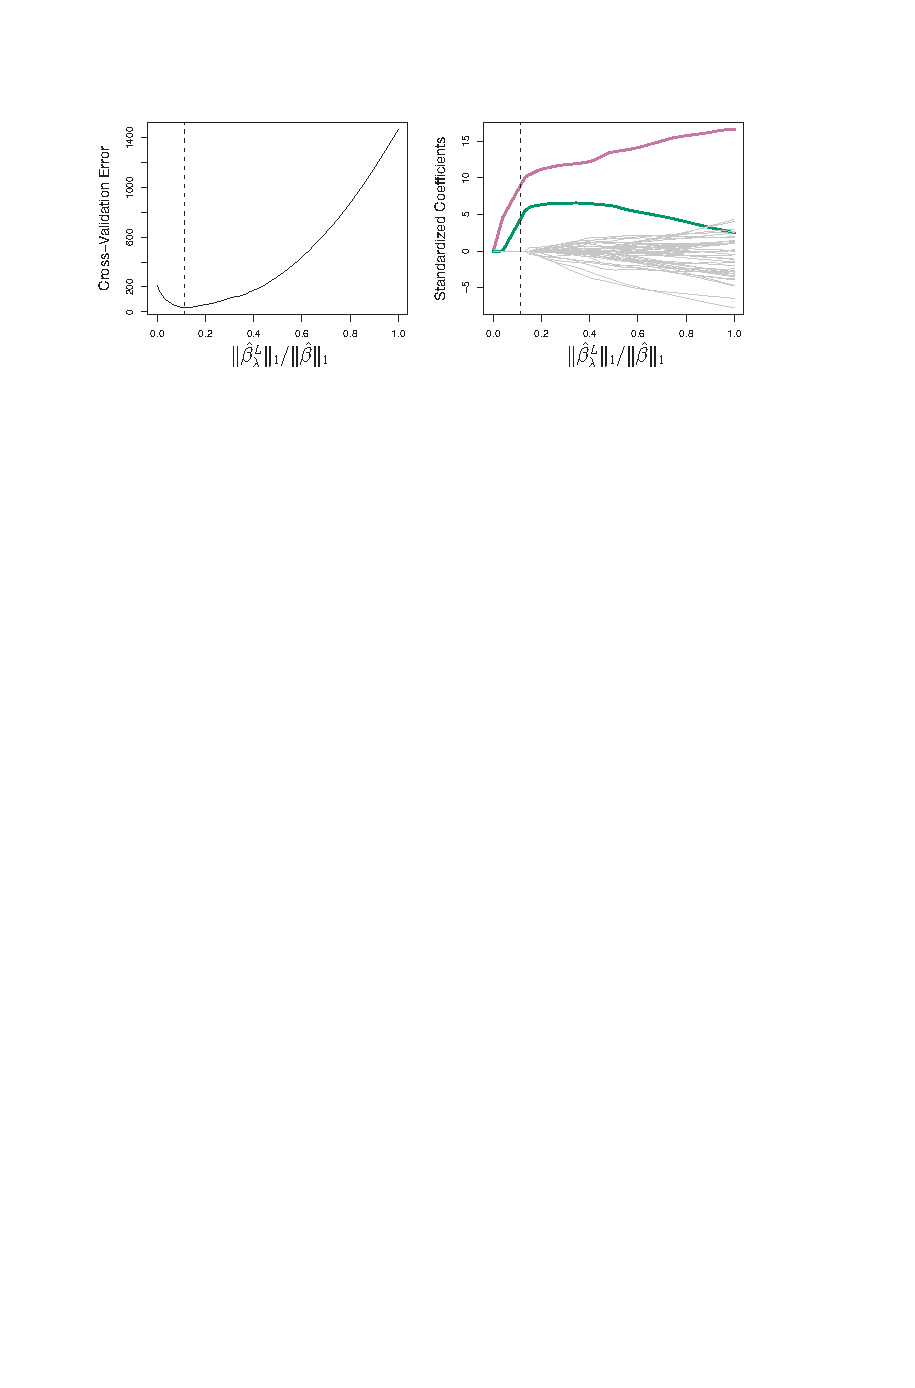
\includegraphics[scale=.7]{lasso-tenfold}
\end{figure}

\pause

Simple $\lambda$ selection strategy: use k-fold cross validation to test performance on a grid of $\lambda$ values. 


\end{frame}

\begin{frame}{Normalizing variables}

It's usually good practice to "normalize" your variables:

\begin{equation}
x' = \frac{x - \bar{x}}{\sigma_x}
\end{equation}

...and then fit the model to the normalized values.  \\~\\

Any guesses why?\\~\\

\pause

Reason: This way variables with large numeric values don't dominate the solution.  

\end{frame}

\begin{frame}{Hot topic:  Elastic nets...}

\begin{columns}
\column{0.5\textwidth}
...are cool!\\~\\

Elastic nets
\begin{itemize}
\item Drive parameters to zero like lasso
\item Deals with correlated predictors well, like ridge (by shinking them together)
\item Give you another !\&@!\%* parameter to tune
\item Still aren't always best -- good to try several shrinkage methods, not just this.
\end{itemize}

\column{0.5\textwidth}

\begin{align*}
\lambda \sum_{k=1}^K  \left(\alpha \beta_j^2 + (1-\alpha) |\beta_j|\right)
\end{align*}


\begin{figure}
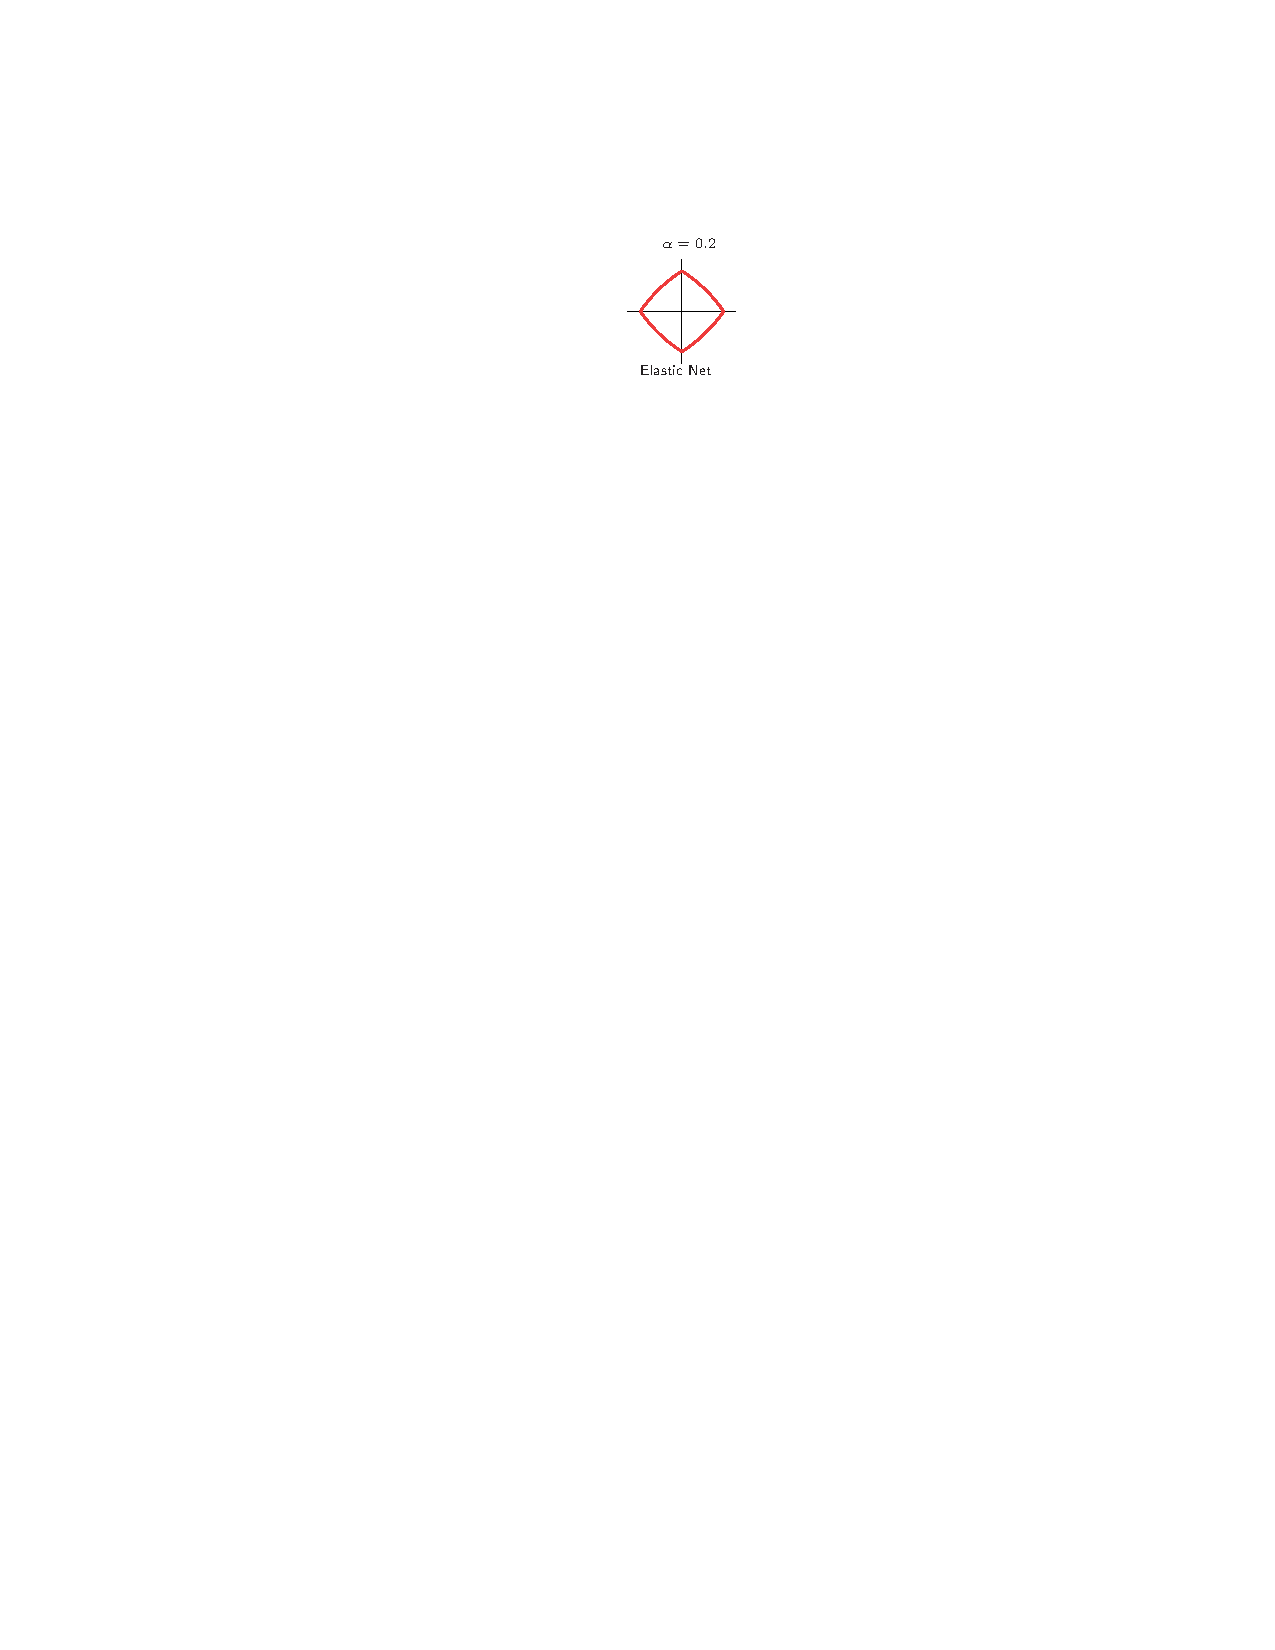
\includegraphics[scale=1]{elastic-net}
\caption*{\tiny from Elements of Statistical Learning}
\end{figure}

\end{columns}
\end{frame}

\begin{frame}
\begin{center}

\Large Dimension Reduction
\end{center}
\end{frame}


\begin{frame}{Principal components analysis (PCA)}

Central idea:  Don't fit the model to your original data!\\~\\

Instead, manufacture a data set $Z_1, Z_2\dots Z_M$ with $M<p$:

\begin{align*}
Z_m= \sum_{j=1}^P \phi_{jm}X_j
\end{align*}

Then fit your model like this:

\begin{align*}
y_i = \theta_0 + \sum_{m=1}^M\theta_{m}z_{im}+\epsilon_i
\end{align*}

...using least squares.\\~\\

If you choose your $\phi$s well (and the data have certain properties, stay tuned), you'll get a lower dimension model than standard regression with better predictions.  
\end{frame}

\begin{frame}{PCA: Why do it?}

\pause

If $M$ (number of principal components) is less than $p$ (number of original predictors) then you can get similar bias-variance tradeoffs as the shrinkage methods do.  
\end{frame}

\begin{frame}{What are these components, anyway?}

Textbook example: using spending on advertising and market population to predict sales.  \\~\\

The figure below shows two components plotted against the original predictors.  

\begin{figure}
\includegraphics[scale=0.8]{pca-ad-vs-pop}
\end{figure}

Note: using two components on a 2-D data set defeats the purpose of PCA (no dimension reduction), but the example is instructive (I hope).
\end{frame}

\begin{frame}{What are these components, anyway?}

\begin{figure}
\includegraphics[scale=0.8]{pca-ad-vs-pop}
\end{figure}

The first component (green) is a line through the data such that 

\begin{align*}
\text{var}\left(\phi_{11}\times (\texttt{pop} - \overline{\texttt{pop}})+ \phi_{21}\times (\texttt{ad} - \overline{\texttt{ad}})\right)
\end{align*}
is maximized.
\end{frame}

\begin{frame}{Projecting onto the component}

\begin{figure}
\includegraphics[scale=1]{pca-ad-vs-pop-projections}
\end{figure}

\begin{align*}
Z_1 = 0.839\times (\texttt{pop} - \overline{\texttt{pop}})+ 0.544\times (\texttt{ad} - \overline{\texttt{ad}})\\
%
z_{i1} = 0.839\times (\texttt{pop}_i - \overline{\texttt{pop}})+ 0.544\times (\texttt{ad}_i - \overline{\texttt{ad}})
\end{align*}
\end{frame}

\begin{frame}{A totally cool way of seeing the variance of the projections...}

...is here:


\url{https://stats.stackexchange.com/questions/2691/making-sense-of-principal-component-analysis-eigenvectors-eigenvalues}
\end{frame}

\begin{frame}{A really important point}
By maximizing variance of the projected values, PCA is finding a component loading that minimizes distance between the line and the predictor.\\~\\

This is sort of like regression, but different:
\begin{itemize}
\item It's minimizing the perpendicular distance to the line, not just the vertical (y-axis) distance
\item It's not doing anything with the response variable ($y$).  \textit{It's just looking for correlation between predictors. }
\end{itemize}
\end{frame}

\begin{frame}{How do you find the components?}
\textit{Option 1}: Let R do it.\\~\\

\pause

\textit{Option 2}: realize that the directions of the components each correspond to one of the \textit{eigenvectors} of the $X^TX$ matrix.  \\~\\

Recall (perhaps?) that the eigenvectors $\mathbf{v}$ and eigenvalues $\lambda$ of a matrix $A$ satisfy:
\begin{align*}
A\mathbf{v} = \lambda \mathbf{v}
\end{align*}

The eigenvector associated with the largest eigenvalue is the direction of the first component.  \\~\\

Note, the eigenvector defines a direction only.  PCA typically sets $\phi$ values such that they describe the direction of the eigenvector \textit{and} satisfy $\sum_{j=1}^p \phi_{ij}^2 = 1$

\end{frame}



\begin{frame}{Why do PCA?}

\begin{columns}

\column{0.55\textwidth}
PCA works when the directions in which $X_1, X_2,\dots X_p$ show the most variation are associated with $Y$.  \

\vspace*{2mm}

That helps us to mitigate overfitting: we use a smaller number of predictors than in the original data. 

\vspace*{2mm}

In this example the data are scarcely correlated with the second component.
\column{0.45\textwidth}

\includegraphics[scale=0.9]{second-vs-first-component}

\end{columns}

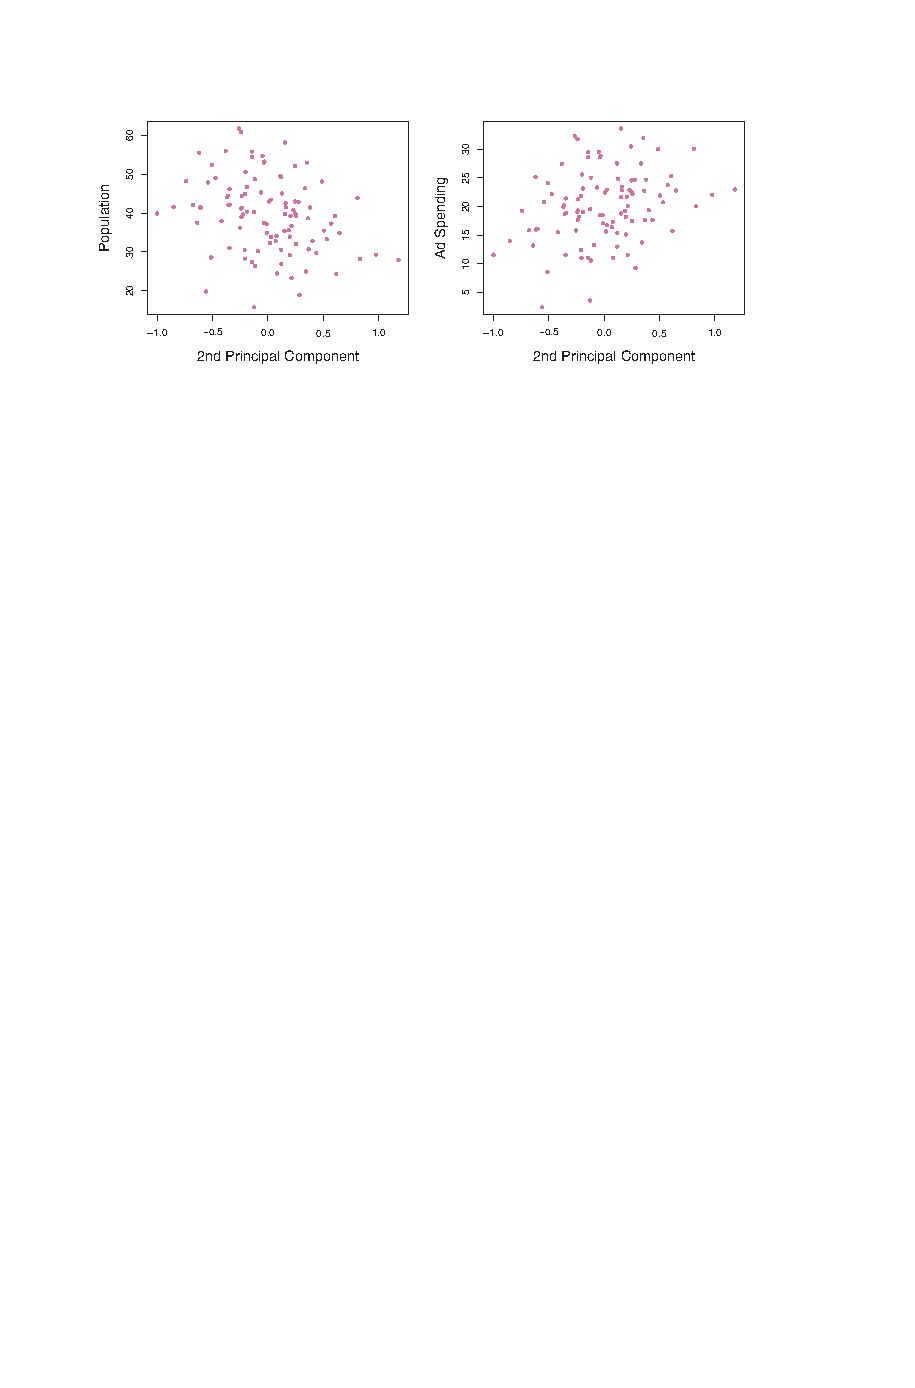
\includegraphics[scale=0.9]{ad-or-spend-vs-second-comp}
\end{frame}


\begin{frame}{Let's see textbook example -- this time PCA, not shinkage}

\begin{columns}
\column{0.5\textwidth}
Simulated data: $n=50$ and $p=45$; response is a function of all 45 predictors. 
\begin{figure}
\includegraphics[scale=0.9]{PCA-45variables}
\end{figure}

\column{0.5\textwidth}
Simulated data: $n=50$ and $p=45$; response is a function of only 2 of the 45 predictors.  
\begin{figure}
\includegraphics[scale=0.9]{PCA-2variables}
\end{figure}

\end{columns}


Q: Why don't we see the error drop down for 2 components on the right?  

\vspace{2mm}

\pause

A: If the two key predictors are not strongly correlated with others, PCA won't find them.  

\vspace{2mm}

Lesson: PCA chooses correlated $X$s.  These may not predict the response.

\end{frame}



\begin{frame}{Setting up Kleinberg \textit{et al}}

$X_0$: Inputs a regulator can manipulate.  A rain dance; an umbrella.  \\
$X$: other inputs\\
$Y$: outcomes\\
$\pi(X_0,Y)$: a ``payoff'' function.  Think of this as social welfare.\\~\\

Question: how much can I improve welfare by changing $X_0$?

\begin{align*}
\frac{d\pi(X_0,Y)}{d X_0} = \frac{\partial \pi}{\partial X_0}(Y) + \frac{\partial \pi}{\partial Y}\frac{\partial Y}{\partial X_0}  
\end{align*}

\pause
First term: how much payoff to taking an action changes as the outcome changes\\~\\

\pause
Second term: how much changing the outcome changes welfare. 

\end{frame}

\begin{frame}{A little more Kleinberg \textit{et al}}

\begin{align*}
\frac{d\pi(X_0,Y)}{d X_0} = \frac{\partial \pi}{\partial X_0}(Y) + \frac{\partial \pi}{\partial Y}\frac{\partial Y}{\partial X_0}  
\end{align*}

\vspace{5mm}

Which term requires causal inference?  Which term requires pure prediction?  
\end{frame}

\begin{frame}{For Thursday}

\begin{enumerate}
\item Read Kleinberg \textit{et al}, and Read Athey Science.  
\item Come to class with ideas for two umbrella policies and two rain dance policies, and two the span between.  Have them relate to the course topic -- energy, ej, access.  
\item In class, discuss if and how your data set might be useful for addressing one of these types of problems.  
\end{enumerate}
\end{frame}







\end{document}
